% section: 応用7パターン

\section{応用7パターン}
  ここからは,いかにして基本4パターンに帰着させるか,という話をしていく.
  つまりは \ref{sec:before} でいう"きれい"な形を目指すということである.
  問題を解くときには,いかにして既知の形にするか,いかにして単純な形にするかを考える.
  漸化式で言えば,基本4パターンがそれに該当する.
  この形であれば解けるというのを1つづつ増やしていき,それらを積み重ねる.
  漸化式,ひいては数学において重要なことである.
  
% subsection: 特性方程式型 \, $a_{n+1}=pa_n+q$

  \subsection{特性方程式型 \, $a_{n+1}=pa_n+q$}
    応用パターンの1つ目,特性方程式型について説明する.
    まずは一般的な形を見せよう.
    \[
      a_{n+1}=pa_n+q
    \]
    さて,この漸化式はどのように解くことができるだろうか.
    数学の問題を解くときの強い原則は,知っている形にすることである.
    ここでも同じで,漸化式をうまく変形して知っている形に変形できれば解くことができる.
    
    そこから考えて,先に扱った基本4パターンの知識を使ってこの漸化式を分析してみよう.
    この漸化式は$a_n$に対して$p$が掛けられ,さらに$q$が足されている.
    つまり,この漸化式は,等比型と階差型の組み合わせからなっていることがわかる.
    そこから判断して,ここは少々突飛な発想ではあるが,この漸化式を等比型に帰着させることを試みよう.
    
    この漸化式は,等比型漸化式
    \[
      a_{n+1}=pa_n
    \]
    に対して$q$が足されたものだ.
    つまりは,\,$q$がうまく消えてくれるような計算式を考えたいのだ.
    その分だけうまく戻せばよい.
    結論から言えば,
    \[
      \begin{array}{rrl}
         & a_{n+1}={} & pa_n+q\\
        -\,) & \alpha={} & p\alpha+q\\ \hline
         & a_{n+1}-\alpha={} & p(a_n-\alpha)
      \end{array}
    \]
    より,
    \[
      a_{n+1}-\alpha=p(a_n-\alpha)
    \]
    を満たすような$\alpha$を考えればよい.
    この式を特性方程式と言う.
    形式的には,
    \[
      a_{n+1}-\alpha=p(a_n-\alpha)
    \]
    または
    \[
      \alpha=p\alpha+q
    \]
    を解き,\,$\alpha$を求めればよい.
    続けると,
    \begin{align*}
      &a_{n+1}-\alpha=p(a_n-\alpha)\\
      &a_{n+1}-\alpha=pa_n-p\alpha\\
      &a_{n+1}=pa_n-p\alpha+\alpha\\
      &a_{n+1}=pa_n+(1-p)\alpha
    \end{align*}
    $(1-p)\alpha$について,
    \[
      a_{n+1}=pa_n+q
    \]
    と係数比較を行うと,
    \begin{align*}
      &q=(1-p)\alpha\\
      &\therefore \quad \alpha=\frac{q}{1-p}
    \end{align*}
    $\alpha$が求まったので,次のステップに移る.
    式の見た目を整えるために,\,$b_n=a_n-\alpha$と置く.
    すると,
    \begin{align*}
      &a_{n+1}-\alpha=p(a_n-\alpha) \iff b_{n+1}=pb_n
    \end{align*}
    この等比型漸化式$b_{n+1}=pb_n$を解くと,
    \begin{align*}
      &b_{n+1}=pb_n\\
      &\therefore \quad b_n=b_1p^{n-1}\\
      &a_n-\alpha=(a_1-\alpha)p^{n-1}\\
      &a_n=(a_1-\alpha)p^{n-1}+\alpha\\
      &\therefore \quad a_n=\left(a_1-\frac{q}{1-p}\right)p^{n-1}+\frac{q}{1-p}
    \end{align*}
    となり,\,$a_n$の一般項が示された.
    やってほしくないことは,この議論の末に得られた結果の形だけを覚えて問題に挑むことである.
    この議論全体を問題を解くたびに都度再現してほしい.

    もう少し数学の世界に深入りしていこう.
    \,$\alpha$を求めるというのはどういった意味合いを持つだろうか.
    漸化式を
    \[
      a_{n+1}=f(a_n)
    \]
    と考え,
    \[
      y=f(x)=px+q
    \]
    について,\,$y=x$との交点,すなわち
    \[
      f(a_{n+1})=f(a_n)
    \]
    を満たすような不動点を考える.図示すると

    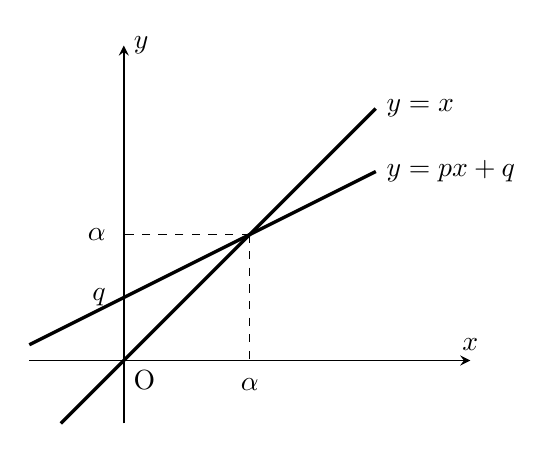
\begin{tikzpicture}[scale=0.8]
      \draw[->,>=stealth,semithick] (-1.5,0)--(5.5,0)node[above]{$x$};
      \draw[->,>=stealth,semithick] (0,-1)--(0,5)node[right]{$y$};
      \draw (0,0)node[below right]{O};

      \draw[very thick,domain=-1:4]
        plot(\x,\x)node[right]{$y=x$};

      \draw[very thick,domain=-1.5:4]
        plot(\x,\x/2+1) node[right] {$y=px+q$};

      % q
      \node[left=3pt] at (0,1) {$q$};

      % 交点から各軸へ点線
      \draw[dashed] (2,2) -- (2,0);
      \draw[dashed] (2,2) -- (0,2);

      % α
      \node[below=3pt] at (2,0) {$\alpha$};
      \node[left=3pt] at (0,2) {$\alpha$};
    \end{tikzpicture}

    というような状況である.
    この交点$(\alpha,\alpha)$を原点と思ってグラフをみると,この座標平面は$y=px$と$y=x$のグラフが原点から始まって進んでいくようなものに見える.
    言い換えれば等比型漸化式に帰着させたということである.
    このような点$(\alpha,\alpha)$を不動点という.

    この不動点を知ることによって,複雑な値の変化をより簡素な値の変化に置き換えることができる.
    また,この話から,漸化式の作る値はのおよその大きさは,\,$p$が作るということが分かる.
    \,$a_n$に対しての和で影響を与える$q$によってもたらされる値の変化より,\,$a_n$に対して積で影響を与える$p$によってもたらされる値の変化の方がはるかに大きいからだ.

    また,特性方程式型漸化式には別の解法が存在する.
    以下に示す.
    \begin{align*}
      &a_{n+1}=pa_n+q \tag*{\(\cdots\) (1)}\\
      &a_{n+2}=pa_{n+1}+q \tag*{\(\cdots\) (2)}\\
    \end{align*}
    $(2)-(1)$をし
    \[
      a_{n+2}-a_{n+1}=p(a_{n+1}-a_n)
    \]
    ここで,\,$b_n=a_{n+1}-a_n$と置くと,
    \begin{align*}
      &b_{n+1}=pb_n
    \end{align*}
    このようにすることで,漸化式は等比数列に帰着する.
    この後の処理は読者に委ねる.

    こちらの図形的解釈は先程の交点を考えるものとは違い,今度は平行な直線を考えることに該当する.
    先程の議論から,\,$p$の情報が欠けた式はその漸化式から生まれる一般項の様相を大きく変えてしまうことがわかる.
    したがってこの場合では$y=x$の代わりに$y=px$を用いる.
    これらの前提を元に図示すると

    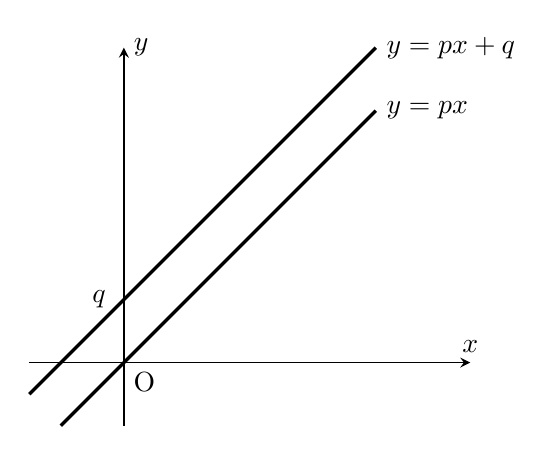
\begin{tikzpicture}[scale=0.8]
      \draw[->,>=stealth,semithick] (-1.5,0)--(5.5,0)node[above]{$x$};
      \draw[->,>=stealth,semithick] (0,-1)--(0,5)node[right]{$y$};
      \draw (0,0)node[below right]{O};

      \draw[very thick,domain=-1:4]
        plot(\x,\x)node[right]{$y=px$};

      \draw[very thick,domain=-1.5:4]
        plot(\x,\x+1) node[right] {$y=px+q$};

      % q
      \node[left=3pt] at (0,1) {$q$};

    \end{tikzpicture}
    
    常に関数の差が$q$と一定になっていることが図からわかる.

    今後,特性方程式を用いた解法を多数扱う.
    特性方程式は漸化式を解く中で重要な概念なのである.
    その背景には行列や線形代数が深く絡んでいる.

  \noindent \textbf{【例題】}
  \begin{enumerate}[label=(\arabic*),parsep=3pt]
    \item $\displaystyle a_1=1,\, a_{n+1}=2a_n+1$
    \item $\displaystyle a_1=1,\, a_{n+1}=\frac{1}{2}a_n+2$
    \item $\displaystyle a_1=1,\, a_{n+1}=a_n+2$
  \end{enumerate}

  \noindent\textbf{【方針】}
  \begin{enumerate}[label=(\arabic*),parsep=3pt]
    \item まずは,\,$\alpha$を求めて等比型に帰着させる方法で解きましょう.
    \item 同じく,\,$\alpha$を求めて等比型に帰着させる方法で解きましょう.
    \item この漸化式は等差型ですが,試しに特性方程式型に帰着させることを考えてみましょう.\,$\alpha$は存在しますか?
  \end{enumerate}

  \noindent\textbf{【解答】}
  \begin{enumerate}[label=(\arabic*),parsep=3pt]
    \item $\displaystyle a_n=2^n-1$
    \item $\displaystyle a_n=4-3\cdot\left(\frac{1}{2}\right)^{n-1}$
    \item $\displaystyle a_n=1+2(n-1)$
  \end{enumerate}

  \noindent\textbf{【解法】}
  \begin{enumerate}[label=(\arabic*),parsep=3pt]
    \item $\displaystyle a_1=1,\,a_{n+1}=2a_n+1$\\
          特性方程式を考えると,
          \[
            \alpha=2\alpha+1
            \quad\Longleftrightarrow\quad
            \alpha=-1
          \]
          である.

          $b_n=a_n-\alpha=a_n+1$とおくと,
          \begin{align*}
            b_{n+1}
              &=a_{n+1}+1\\
              &=2a_n+2\\
              &=2(a_n+1)\\
              &=2b_n.
          \end{align*}
          また,\,$b_1=a_1+1=2$であるから,
          \[
            b_n=2^n.
          \]
          よって,
          \[
            a_n=b_n-1=2^n-1.
          \]

    \item $\displaystyle a_1=1,\,a_{n+1}=\frac12a_n+2$\\
            特性方程式を考えると,
            \[
              \alpha=\frac12\alpha+2
              \quad\Longleftrightarrow\quad
              \alpha=4
            \]
            である.

            $b_n=a_n-\alpha=a_n-4$とおくと,
            \begin{align*}
              b_{n+1}
                &=a_{n+1}-4\\
                &=\frac12a_n+2-4\\
                &=\frac12(a_n-4)\\
                &=\frac12b_n.
            \end{align*}
            また,\,$b_1=a_1-4=-3$であるから,
            \[
              b_n=-3\left(\frac12\right)^{n-1}.
            \]
            よって,
            \[
              a_n=b_n+4
              =4-3\left(\frac12\right)^{n-1}.
            \]
     \item $\displaystyle a_1=1,\, a_{n+1}=a_n+2$\\
           $\alpha$は存在しないので,特性方程式型に帰着させることはできない.
           これが意味することは,不動点を持たないということである.
  \end{enumerate}


\input{第3章 漸化式の解説/05_応用7パターン/02_階差等比複合型/階差等比複合型.tex}
% subsection: 対数型 \, $a_{n+1}=pa_n^q$

  \subsection{対数型 \, $a_{n+1}=pa_n^q$}
    今までは$a_n$に対する操作は定数倍したり関数が掛けられたりするだけだった.
    しかし,\,$a_n$に指数がついたらどうだろうか.
    この場合はかなり難しい発想の変形が必要である.
    それは対数を取るという操作である.
    実際にやってみよう.
    \[
      a_{n+1}=pa_n^q
    \]
    について,両辺の対数を取ると
    \begin{align*}
      \log_p{a_{n+1}}&=\log_p{pa_n^q}\\
      &=\log_p{p}+\log_p{a_n^q}\\
      &=q\log_p{a_n}+1
    \end{align*}
    $b_n=\log_p{a_n}$とおくと,
    \begin{align*}
      b_{n+1}=qb_n+1
    \end{align*}
    あとはただの特性方程式型の問題である.
    底をいくらにするかは自由だが$p$に関連する数だと扱いやすい.
    たとえば$p=k^m$の時は$k$でとっておくことが多い.
    作問者側は解答がシンプルな形になるようにするため,より小さい底を取ることで答えが求めやすくなる.

    また,対数の強みは積を和に,商を差にできるところにある.
    漸化式が全て積や商のみで表される場合にその強みが現れる.
    これはここで解説するよりも演習問題を通して経験するほうがわかりやすいと判断したため,この内容は(2)で取り扱っている.
  
    \noindent\textbf{【例題】}
    \begin{enumerate}[label=(\arabic*),parsep=3pt]
      \item $\displaystyle a_1=2,\quad a_{n+1}=2a_n^2$
      \item $\displaystyle a_1=\frac{1}{2},\quad a_{n+1}=\frac{1}{a_n}$
      \item $\displaystyle a_1=1,\quad a_{n+1}=(n+1)a_n$
      \item $\displaystyle a_1=5,\quad a_{n+1}=a_n^2-2a_n+2$
    \end{enumerate}

    \noindent\textbf{【方針】}
    \begin{enumerate}[label=(\arabic*),parsep=3pt]
      \item 両辺の底を$2$とする対数を取り,\,$b_n=\log_2a_n$とおいて一次の漸化式に変形します.その結果,漸化式は特性方程式型になります.
      \item 一見すると分数型(後述)のように見えますが,対数型として解くことができます.
      \item 階比型に見えますが,対数型としても解けます.
      \item うまく変形すると対数型になります.
    \end{enumerate}

    \noindent\textbf{【解答】}
    \begin{enumerate}[label=(\arabic*),parsep=3pt]
      \item $\displaystyle a_n=2^{3\cdot2^{n-1}-2}$
      \item $a_n=2^{(-1)^{n}}$
      \item $a_n=n!$
      \item $a_n=2^{2^n}+1$
    \end{enumerate}

    \noindent\textbf{【解法】}
    \begin{enumerate}[label=(\arabic*),parsep=3pt]
      \item $\displaystyle a_1=2,\quad a_{n+1}=2a_n^2$\\
            両辺の底を$2$とする対数を取ると,
            \begin{align*}
              \log_2a_{n+1}
                &=\log_2{2a_n^2}\\
                &=2\log_2{2a_n}\\
                &=2(\log_2{2}+\log_2{a_n})\\
                &=2\log_2{a_n}+2
            \end{align*}
            ここで
            \[
              b_n=\log_2a_n
            \]
            とおくと,
            \begin{align*}
              &b_{n+1}=2b_n+2\\
              &b_{n+1}+2=2(b_n+2)
            \end{align*}
            ここで
            \[
              c_n=b_n+2
            \]
            とおくと,
            \[
              c_{n+1}=2c_n
            \]
            $c_1$は,
            \[
              c_1=b_1+2=\log_2{a_1}+2=\log_2{2}+2=1+2=3
            \]
            従って,
            \begin{align*}
              &c_n=3\cdot2^{n-1}\\
              &b_n+2=3\cdot2^{n-1}\\
              &b_n=3\cdot2^{n-1}-2\\
              &a_n=2^{3\cdot2^{n-1}-2}
            \end{align*}
      \item $\displaystyle a_1=2,\quad a_{n+1}=\frac{1}{a_n}$\\
            与式の両辺の底を2とする対数を取ると,
            \begin{align*}
              &\log_2{a_{n+1}}=\log_2{\frac{1}{a_n}}\\
              &\log_2{a_{n+1}}=\log_2{1}-\log_2{a_n}\\
              &\log_2{a_{n+1}}=-\log_2{a_n}\\
              &\log_2{a_n}=\log_2{a_1}(-1)^{n-1}\\
              &\log_2{a_n}=\log_2{\frac{1}{2}}(-1)^{n-1}\\
              &\log_2{a_n}=(-1)^{n}\\
              &\therefore \quad a_n=2^{(-1)^{n}}
            \end{align*}
      \item $\displaystyle a_1=1,\quad a_{n+1}=(n+1)a_n$\\
            両辺の自然対数を取って
            \[
              \log a_{n+1}=\log{n+1}+\log a_n
            \]
            したがって
            \begin{align*}
              \log a_n&=\log a_1 + \log{2}+\cdots+ \log{n}\\
              &=\log 1 + \log{2}+\cdots +\log{n}\\
              &=\log n!\\
              &\therefore \quad a_n=n!
            \end{align*}
      \item $\displaystyle a_1=5,\quad a_{n+1}=a_n^2-2a_n+2$\\
            与式を変形して
            \[
              a_{n+1}-1=(a_n-1)^2
            \]
            両辺の底を2とする対数を取ると,
            \begin{align*}
              &\log_2{(a_{n+1}-1)}=\log_2{(a_n-1)^2}\\
              &\log_2{(a_{n+1}-1)}=2\log_2{(a_n-1)}\\
              &\log_2{(a_n-1)}=2^{n-1}\cdot\log_2{(a_1-1)}\\
              &\log_2{(a_n-1)}=2^{n-1}\cdot\log_2{4}\\
              &\log_2{(a_n-1)}=2^{n}\\
              &a_n-1=2^{2^{n}}\\
              &\therefore \quad a_n=2^{2^{n}}+1
            \end{align*}
    \end{enumerate}
    \noindent\textbf{【補足】}

    (3)では底をネイピア数としたが,底は任意の値で構わない.


\input{第3章 漸化式の解説/05_応用7パターン/04_分数型/分数型.tex}
\input{第3章 漸化式の解説/05_応用7パターン/05_隣接3項間漸化式型/隣接3項間漸化式型.tex}
% subsection: 総和型

  \subsection{総和型}
    \subsubsection{総和と一般項の漸化式型 \, $S_n=pa_n+f(n)$}
      ある漸化式によって定められる数列$a_n$によって,
      \[
        S_n=\sum_{k=1}^{n} a_k
      \]
      として定められる数列$S_n$について考えよう.
      $S_n$と$a_n$の関係を表した
      \[
        S_n=pa_n+f(n)
      \]
      のような漸化式を考える.
      このような漸化式は今まで取り扱った形にはない,未知のものである.
      であれば既知の形にするのが数学である.
      これまでのことをきちんと理解していれば,\,$a_{n+1}$と$a_n$の関係が分かっている時には解くことができる.
      $S_n$をうまく変形して$a_{n}$関連だけの式を産むには,\,$p \neq 1$の時,
      \begin{align*}
        &S_n=pa_n+f(n) \tag*{\(\cdots\) (1)}\\
        &S_{n+1}=pa_{n+1}+f(n+1) \tag*{\(\cdots\) (2)}
      \end{align*}
      $(2)-(1)$をして
      \begin{align*}
        &a_{n+1}=pa_{n+1}-pa_n+f(n+1)-f(n)\\
        &a_{n+1}-pa_{n+1}=-pa_n+f(n+1)-f(n)\\
        &a_{n+1}(1-p)=-pa_n+f(n+1)-f(n)\\
        &a_{n+1}=\frac{-pa_n+f(n+1)-f(n)}{(1-p)}\\
        &a_{n+1}=\frac{p}{p-1}a_n+\frac{1}{1-p}\{f(n+1)-f(n)\}
      \end{align*}
      $\displaystyle g(n)=\frac{1}{1-p}\{f(n+1)-f(n)\}$とおくと,
      \begin{align*}
        &a_{n+1}=\frac{p}{p-1}a_n+g(n)
      \end{align*}
      従って漸化式は階差数列型に帰着する.\,$p=1$のときも同様の流れで求めることができる.

      \noindent \textbf{【例題】}
      \begin{enumerate}[label=(\arabic*),parsep=3pt]
        \item $\displaystyle S_n=2a_n-n$
        \item $\displaystyle S_n=\frac12a_n+n$
      \end{enumerate}

      \noindent\textbf{【方針】}
      \begin{enumerate}[label=(\arabic*),parsep=3pt]
        \item まず$n=1$を代入して$a_1$を求めてから,本文の変形をなぞって$a_{n+1}$と$a_n$だけの漸化式を作りましょう.
        \item 同様です.できた漸化式は特性方程式型に帰着します.
      \end{enumerate}

      \noindent\textbf{【解答】}
      \begin{enumerate}[label=(\arabic*),parsep=3pt]
        \item $\displaystyle a_n=2^n-1$
        \item $\displaystyle a_n=1+(-1)^{n-1}$
      \end{enumerate}

      \noindent\textbf{【解法】}
      \begin{enumerate}[label=(\arabic*),parsep=3pt]
      \item $\displaystyle S_n=2a_n-n$

          $n=1$を代入すると,
          \[
            S_1=a_1=2a_1-1
          \]
          より
          \[
            a_1=1
          \]
          また,
          \begin{align*}
            a_{n+1}
              &=S_{n+1}-S_n\\
              &=\{2a_{n+1}-(n+1)\}-(2a_n-n)\\
              &=2a_{n+1}-2a_n-1.
          \end{align*}
          したがって,
          \[
            a_{n+1}=2a_n+1.
          \]
          ここで $b_n=a_n+1$ とおくと,
          \begin{align*}
            b_{n+1}
              &=a_{n+1}+1\\
              &=2a_n+2\\
              &=2(a_n+1)\\
              &=2b_n.
          \end{align*}
          また,
          \[
            b_1=a_1+1=2
          \]
          であるから,
          \[
            b_n=2^n.
          \]
          よって,
          \[
            a_n=2^n-1.
          \]
      \item $\displaystyle S_n=\frac12a_n+n$
          $n=1$を代入すると,
          \[
            S_1=a_1=\frac12a_1+1
          \]
          より
          \[
            a_1=2
          \]
          \begin{align*}
            a_{n+1}
              &=S_{n+1}-S_n\\
              &=\left\{\frac12a_{n+1}+(n+1)\right\}-\left(\frac12a_n+n\right)\\
              &=\frac12a_{n+1}-\frac12a_n+1.
          \end{align*}
          したがって,
          \[
            a_{n+1}=-a_n+2.
          \]

          ここで $b_n=a_n-1$ とおくと,
          \begin{align*}
            b_{n+1}
              &=a_{n+1}-1\\
              &=-a_n+1\\
              &=-(a_n-1)\\
              &=-b_n.
          \end{align*}
          また,
          \[
            b_1=a_1-1=1
          \]
          であるから,
          \[
            b_n=(-1)^{n-1}.
          \]
          よって,
          \[
            a_n=1+(-1)^{n-1}.
          \]

      \end{enumerate}

    \subsubsection{純総和型 \, $S_{n+1}=pS_n+f(n) $}
      両辺に総和がきてもやることは一緒で,1つずらした総和と元の式を足し引きしてやることで,\,$a_n$や$a_{n+1}$の項を作れば良い.
      \begin{align*}
        &S_{n+1}=pS_n+f(n) \tag*{\(\cdots\) (1)}\\
        &S_{n}=pS_{n-1}+f(n-1) \tag*{\(\cdots\) (2)}\\
      \end{align*}
        $(1)-(2)$をして,
      \begin{align*}
        &a_{n+1}=pa_{n}+f(n)-f(n-1)
      \end{align*}
      あとはただの階差数列型の計算である.

      \noindent \textbf{【例題】}
      \begin{enumerate}[label=(\arabic*),parsep=3pt]
        \item $\displaystyle S_1=1,\ S_{n+1}=2S_n+n$
      \end{enumerate}

      \noindent\textbf{【方針】}
      \begin{enumerate}[label=(\arabic*),parsep=3pt]
        \item 本文の式は$n\ge2$でしか使えないことに注意し,\,$a_2$だけは$S_2=2S_1+f(1)$から別に求めましょう.
      \end{enumerate}

      \noindent\textbf{【解答】}
      \begin{enumerate}[label=(\arabic*),parsep=3pt]
        \item $\displaystyle a_1=1,\quad a_n=3\cdot2^{n-2}-1\ (n\ge2)$
      \end{enumerate}

      \noindent\textbf{【解法】}
      \begin{enumerate}[label=(\arabic*),parsep=3pt]
      \item $\displaystyle S_1=1,\ S_{n+1}=2S_n+n$
          $a_1=S_1=1$である.
          また,
          \begin{align*}
            &S_{n+1}=a_1+a_2+\cdots+a_n+a_{n+1}\\
            &S_n=a_1+a_2+\cdots+a_n
          \end{align*}
          であるから,
          \[
            S_{n+1}-S_n=a_{n+1}.
          \]
          したがって,
          \begin{align*}
            a_{n+1}
              &=S_{n+1}-S_n\\
              &=(2S_n+n)-S_n\\
              &=S_n+n.
          \end{align*}
          ここで,
          \[
            S_n=2S_{n-1}+(n-1)
          \]
          より,
          \begin{align*}
            a_{n+1}
              &=2S_{n-1}+(n-1)+n\\
              &=2S_{n-1}+2n-1.
          \end{align*}
          一方,
          \[
            a_n=S_n-S_{n-1}
          \]
          であるから,
          \[
            S_n=2S_{n-1}+(n-1)
          \]
          を用いて,
          \[
            a_n=S_{n-1}+n-1,
          \]
          したがって
          \[
            S_{n-1}=a_n-(n-1).
          \]
          これを上式に代入すると,
          \begin{align*}
            a_{n+1}
              &=2\{a_n-(n-1)\}+2n-1\\
              &=2a_n+1.
          \end{align*}

          なお,\,$n=1$のときは
          \[
            a_2=S_2-S_1=(2S_1+1)-S_1=2
          \]
          であり,上の漸化式
          \[
            a_{n+1}=2a_n+1
          \]
          は$n\ge1$で成り立つ.

          ここで $b_n=a_n+1$ とおくと,
          \begin{align*}
            b_{n+1}
              &=a_{n+1}+1\\
              &=2a_n+2\\
              &=2(a_n+1)\\
              &=2b_n.
          \end{align*}
          また,
          \[
            b_1=a_1+1=2
          \]
          であるから,
          \[
            b_n=2^n.
          \]
          よって,
          \[
            a_n=2^n-1.
          \]
      \end{enumerate}


% subsection: 連立型

\subsection{連立型}
  \subsubsection{加減法型}
    一般形が
    \[
      \begin{cases}
        a_{n+1}=pa_{n}+qb_{n} \\
        b_{n+1}=qa_{n}+pb_{n}
      \end{cases}
    \]
    の形で表される漸化式の解き方について考えよう.
    といってもここまで読んだ諸君らにとっては,直感的に与えられた式を足し引きすればいいことが分かるだろう.
    実際にすすめていくと,
    \begin{align*}
      &a_{n+1}+b_{n+1}=(p+q)(a_{n}+b_{n})\\
      &a_n+b_n=(a_1+b_1)(p+q)^{n-1}\tag*{\(\cdots\) (1)}
    \end{align*}
    また,
    \begin{align*}
      &a_{n+1}-b_{n+1}=(p-q)(a_{n}-b_{n})\\
      &a_n-b_n=(a_1-b_1)(p-q)^{n-1}\tag*{\(\cdots\) (2)}
    \end{align*}
    $(1)+(2)$をすると
    \begin{align*}
      &2a_n=(a_1+b_1)(p+q)^{n-1}+(a_1-b_1)(p-q)^{n-1}\\
      &a_n=\frac{(a_1+b_1)(p+q)^{n-1}+(a_1-b_1)(p-q)^{n-1}}{2}\\
    \end{align*}
    $(1)-(2)$をすると
    \begin{align*}
      &2b_n=(a_1+b_1)(p+q)^{n-1}-(a_1-b_1)(p-q)^{n-1}\\
      &b_n=\frac{(a_1+b_1)(p+q)^{n-1}-(a_1-b_1)(p-q)^{n-1}}{2}
    \end{align*}
    別解及び演習は一般型の方で行う.
  \subsubsection{一般型}
    連立一般型の漸化式は,
    \[
      \begin{cases}
        a_{n+1}=pa_{n}+qb_{n} \\
        b_{n+1}=ra_{n}+sb_{n}
      \end{cases}
    \]
    で表される漸化式である.
    いつものように等比数列型への帰着を目指そう.
    $a_n$と$b_n$が互いに影響し合っているため,独立させて解くことは難しそうだ.
    ならばそれぞれについて求めるのではなく,いっそのこと合わせて求めてしまおうというのが解法の思想である.
    その流れは,
    \[
      \begin{array}{rrl}
        & a_{n+1}={} &pa_{n}+qb_{n}\\
        +\,) & b_{n+1}={} & ra_{n}+sb_{n}\\ \hline
        & a_{n+1}+b_{n+1}={} & (p+r)a_{n}+(q+s)b_{n}
      \end{array}
    \]
    について
    \[
      \alpha a_{n+1}+\beta b_{n+1}
      =\gamma(\alpha a_n+\beta b_n)
    \]
    を満たすようにしてやればよい.
    実際に左辺を計算すると,
    \begin{align*}
      \alpha a_{n+1}+\beta b_{n+1}&=\alpha(pa_n+qb_n)+\beta(ra_n+sb_n)\\
      &=(p\alpha+r\beta)a_n+(q\alpha+s\beta)b_n.
    \end{align*}
    一方,
    \[
      \gamma(\alpha a_n+\beta b_n)=\gamma\alpha a_n+\gamma\beta b_n
    \]
    である.
    したがって,
    \[
    \begin{cases}
      p\alpha+r\beta=\gamma\alpha\\
      q\alpha+s\beta=\gamma\beta
    \end{cases}
    \]
    となるように$\alpha,\beta,\gamma$を決めればよい.

    ここで,いきなり3つの文字をすべて求めようとすると少し複雑に見える.
    そこで,まず$\gamma$について考える.

    上の2式を変形すると,
    \[
    \begin{cases}
      (p-\gamma)\alpha+r\beta=0\\
      q\alpha+(s-\gamma)\beta=0
    \end{cases}
    \]
    である.
    $\alpha,\beta$は同時に$0$ではないので,この連立方程式が$\alpha,\beta$について解を持つためには,
    \[
      (p-\gamma)(s-\gamma)-qr=0
    \]
    でなければならない.
    整理すると,
    \[
      \gamma^2-(p+s)\gamma+(ps-qr)=0
    \]
    となる.
    この二次方程式を,この連立漸化式の特性方程式と呼ぶ.
    特性方程式の解を$\gamma_1,\gamma_2$とする.
    まず$\gamma=\gamma_1$を上の連立方程式に代入し,
    \[
      \begin{cases}
        (p-\gamma_1)\alpha+r\beta=0\\
        q\alpha+(s-\gamma_1)\beta=0
      \end{cases}
    \]
    を満たす$\alpha,\beta$を1組求める.
    すると,
    \[
      c_n=\alpha a_n+\beta b_n
    \]
    と置くことで,
    \begin{align*}
      c_{n+1}&=\alpha a_{n+1}+\beta b_{n+1}\\
      &=\gamma_1(\alpha a_n+\beta b_n)\\
      &=\gamma_1c_n
    \end{align*}
    となる.
    したがって,
    \[
      c_n=c_1\gamma_1^{\,n-1}
    \]
    という等比数列が得られる.
    同様に,\,$\gamma=\gamma_2$に対しても$\alpha,\beta$を求めれば,
    \[
      d_n=\alpha' a_n+\beta' b_n
    \]
    について
    \[
      d_n=d_1\gamma_2^{\,n-1}
    \]
    という等比数列が得られる.
    なお,ここで得られた2つの等比数列から$a_n,b_n$を求めるには,
    \[
      \begin{cases}
      c_n=\alpha a_n+\beta b_n\\
      d_n=\alpha'a_n+\beta'b_n
      \end{cases}
    \]
    を$a_n,b_n$について解けばよい.
    このように,\,$a_n,b_n$をそれぞれ直接求めるのではなく,\,$a_n,b_n$の和の形を作ることで,連立していた漸化式を等比数列へと分離することができる.

    \noindent \textbf{【例題】}
    \begin{enumerate}[label=(\arabic*),parsep=3pt]
      \item $\displaystyle a_1=1,\,b_1=1.\ \begin{cases}a_{n+1}=3a_n+b_n\\ b_{n+1}=a_n+3b_n\end{cases}$
      \item $\displaystyle a_1=1,\,b_1=0,\ \begin{cases}a_{n+1}=3a_n+b_n\\ b_{n+1}=2a_n+2b_n\end{cases}$
    \end{enumerate}

    \noindent\textbf{【方針】}
    \begin{enumerate}[label=(\arabic*),parsep=3pt]
      \item 前節で述べた問題です.一般型,加減法型,どちらのやり方でも問題ありません.
      \item これはこの節で述べたものです.
    \end{enumerate}

    \noindent\textbf{【解答】}
    \begin{enumerate}[label=(\arabic*),parsep=3pt]
      \item $\displaystyle a_n=\frac{2\cdot4^{n-1}+1}{3},\qquad b_n=\frac{2\cdot4^{n-1}-2}{3}$
      \item $\displaystyle a_n=4^{n-1},\qquad b_n=a_n=4^{n-1}$
    \end{enumerate}

    \noindent\textbf{【解法】}
    \begin{enumerate}[label=(\arabic*),parsep=3pt]
    \item $\displaystyle a_1=1,\,b_1=1.\ \begin{cases}a_{n+1}=3a_n+b_n\\ b_{n+1}=a_n+3b_n\end{cases}$\\
          \begin{enumerate}
            \item 【解法1】\\
                  $\alpha a_{n+1}+\beta b_{n+1}$を計算すると,
                  \begin{align*}
                    \alpha a_{n+1}+\beta b_{n+1}
                      &=\alpha(3a_n+b_n)\\
                      &\qquad +\beta(a_n+3b_n)\\
                      &=(3\alpha+\beta)a_n\\
                      &\qquad +(\alpha+3\beta)b_n
                  \end{align*}
                  これが
                  \[
                    \gamma(\alpha a_n+\beta b_n)
                    =\gamma\alpha a_n+\gamma\beta b_n
                  \]
                  と一致するためには,
                  \[
                  \begin{cases}
                    (3-\gamma)\alpha+\beta=0\\
                    \alpha+(3-\gamma)\beta=0
                  \end{cases}
                  \]
                  でなければならない.

                  $\alpha,\beta$が同時に$0$ではないため,
                  \[
                    (3-\gamma)^2-1=0
                  \]
                  より,
                  \begin{align*}
                    &\gamma^2-6\gamma+8=0\\
                    &(\gamma-2)(\gamma-4)=0.
                  \end{align*}
                  したがって,
                  \[
                    \gamma_1=2,\qquad\gamma_2=4
                  \]
                  である.

                  まず$\gamma=2$とすると,
                  \[
                  \begin{cases}
                    \alpha+\beta=0\\
                    \alpha+\beta=0
                  \end{cases}
                  \]
                  となるので,
                  \[
                    \alpha=1,\qquad\beta=-1
                  \]
                  と取ることができる.

                  そこで,
                  \[
                    c_n=a_n-b_n
                  \]
                  とおくと,
                  \begin{align*}
                    c_{n+1}
                      &=a_{n+1}-b_{n+1}\\
                      &=(3a_n+b_n)-(a_n+3b_n)\\
                      &=2(a_n-b_n)\\
                      &=2c_n.
                  \end{align*}
                  また,
                  \[
                    c_1=a_1-b_1=0
                  \]
                  であるから,
                  \[
                    c_n=0.
                  \]
                  したがって,
                  \[
                    a_n-b_n=0.
                  \]

                  次に$\gamma=4$とすると,
                  \[
                  \begin{cases}
                    -\alpha+\beta=0\\
                    \alpha-\beta=0
                  \end{cases}
                  \]
                  となるので,
                  \[
                    \alpha=1,\qquad\beta=1
                  \]
                  と取ることができる.

                  そこで,
                  \[
                    d_n=a_n+b_n
                  \]
                  とおくと,
                  \begin{align*}
                    d_{n+1}
                      &=a_{n+1}+b_{n+1}\\
                      &=(3a_n+b_n)+(a_n+3b_n)\\
                      &=4(a_n+b_n)\\
                      &=4d_n.
                  \end{align*}
                  また,
                  \[
                    d_1=a_1+b_1=2
                  \]
                  であるから,
                  \[
                    d_n=2\cdot4^{n-1}.
                  \]

                  以上より,
                  \[
                  \begin{cases}
                    a_n-b_n=0\\
                    a_n+b_n=2\cdot4^{n-1}
                  \end{cases}
                  \]
                  となる.

                  2式を辺々加えると,
                  \[
                    2a_n=2\cdot4^{n-1}
                  \]
                  であるから,
                  \[
                    a_n=4^{n-1}.
                  \]
                  また,
                  \[
                    b_n=a_n=4^{n-1}.
                  \]
            \item 【解法2】\\
                  2つの式を辺々加えると,
                  \begin{align*}
                    a_{n+1}+b_{n+1}
                      &=(3a_n+b_n)\\
                      &\quad +(a_n+3b_n)\\
                      &=4(a_n+b_n)
                  \end{align*}
                  よって,
                  \[
                    a_n+b_n=(a_1+b_1)4^{n-1}=2\cdot4^{n-1}. \tag*{\(\cdots\) (1)}
                  \]

                  また,2つの式を辺々引くと,
                  \begin{align*}
                    a_{n+1}-b_{n+1}
                      &=(3a_n+b_n)\\
                      &\quad -(a_n+3b_n)\\
                      &=2(a_n-b_n)
                  \end{align*}
                  よって,
                  \[
                    a_n-b_n=(a_1-b_1)2^{n-1}=0. \tag*{\(\cdots\) (2)}
                  \]

                  \((1)+(2)\)をすると,
                  \[
                    2a_n=2\cdot4^{n-1}
                  \]
                  なので,
                  \[
                    a_n=4^{n-1}.
                  \]

                  また,\((1)-(2)\)をすると,
                  \[
                    2b_n=2\cdot4^{n-1}
                  \]
                  なので,
                  \[
                    b_n=4^{n-1}.
                  \]
          \end{enumerate}
    \item $\displaystyle a_1=1,\,b_1=0,\ \begin{cases}a_{n+1}=3a_n+b_n\\ b_{n+1}=2a_n+2b_n\end{cases}$\\
          $\alpha a_{n+1}+\beta b_{n+1}$を計算すると,
          \begin{align*}
            \alpha a_{n+1}+\beta b_{n+1}
              &=\alpha(3a_n+b_n)\\
              &\quad +\beta(2a_n+2b_n)\\
              &=(3\alpha+2\beta)a_n\\
              &\quad +(\alpha+2\beta)b_n
          \end{align*}
          これが
          \[
            \gamma(\alpha a_n+\beta b_n)
            =\gamma\alpha a_n+\gamma\beta b_n
          \]
          と一致するためには,
          \[
          \begin{cases}
            (3-\gamma)\alpha+2\beta=0\\
            \alpha+(2-\gamma)\beta=0
          \end{cases}
          \]
          でなければならない.

          $\alpha,\beta$が同時に$0$ではないため,
          \[
            (3-\gamma)(2-\gamma)-2=0
          \]
          より,
          \begin{align*}
            &\gamma^2-5\gamma+4=0\\
            &(\gamma-1)(\gamma-4)=0
          \end{align*}
          したがって,
          \[
            \gamma_1=1,\qquad\gamma_2=4
          \]
          である.

          まず$\gamma=1$とすると,
          \[
          \begin{cases}
            2\alpha+2\beta=0\\
            \alpha+\beta=0
          \end{cases}
          \]
          となるので,
          \[
            \alpha=1,\qquad\beta=-1
          \]
          と取ることができる.

          そこで,
          \[
            c_n=a_n-b_n
          \]
          とおくと,
          \begin{align*}
            c_{n+1}
              &=a_{n+1}-b_{n+1}\\
              &=(3a_n+b_n)-(2a_n+2b_n)\\
              &=a_n-b_n\\
              &=c_n.
          \end{align*}
          また,
          \[
            c_1=a_1-b_1=1
          \]
          であるから,
          \[
            c_n=1.
          \]
          したがって,
          \[
            a_n-b_n=1.
          \]

          次に$\gamma=4$とすると,
          \[
          \begin{cases}
            -\alpha+2\beta=0\\
            \alpha-2\beta=0
          \end{cases}
          \]
          となるので,
          \[
            \alpha=2,\qquad\beta=1
          \]
          と取ることができる.

          そこで,
          \[
            d_n=2a_n+b_n
          \]
          とおくと,
          \begin{align*}
            d_{n+1}
              &=2a_{n+1}+b_{n+1}\\
              &=2(3a_n+b_n)+(2a_n+2b_n)\\
              &=8a_n+4b_n\\
              &=4(2a_n+b_n)\\
              &=4d_n.
          \end{align*}
          また,
          \[
            d_1=2a_1+b_1=2
          \]
          であるから,
          \[
            d_n=2\cdot4^{n-1}.
          \]

          以上より,
          \[
          \begin{cases}
            a_n-b_n=1\\
            2a_n+b_n=2\cdot4^{n-1}
          \end{cases}
          \]
          となる.

          2式を辺々加えると,
          \[
            3a_n=1+2\cdot4^{n-1}
          \]
          であるから,
          \[
            a_n=\frac{2\cdot4^{n-1}+1}{3}.
          \]
          また,
          \[
            b_n=a_n-1
          \]
          より,
          \[
            b_n=\frac{2\cdot4^{n-1}-2}{3}.
          \]
    \end{enumerate}


